\documentclass[
  a4paper,
  oneside,
  BCOR = 10mm,
  DIV = 12,
  12pt,
  headings = normal,
]{scrartcl}

%%% Length calculations
\usepackage{calc}
%%%

%%% Support for color
\usepackage{xcolor}
\definecolor{lightblue}{HTML}{03A9F4}
\definecolor{red}{HTML}{F44336}
%%%

%%% Including graphics
\usepackage{graphicx}
%%%

%%% Font selection
\usepackage{fontspec}

\setromanfont{STIX Two Text}[
  SmallCapsFeatures = {LetterSpace = 8},
]

\setsansfont{IBM Plex Sans}[
  Scale = MatchUppercase,
]

\setmonofont{IBM Plex Mono}[
  Scale = MatchUppercase,
]
%%%

%%% Math typesetting
\usepackage{amsmath}
\usepackage{mathtools}

\usepackage{unicode-math}
\setmathfont{STIX Two Math}

\usepackage{IEEEtrantools}
%%%

%%% List settings
\usepackage{enumitem}
\setlist[enumerate]{
  label*      = {\arabic*.},
  left        = \parindent,
  topsep      = 0\baselineskip,
  parsep      = 0\baselineskip,
  noitemsep, % override itemsep
}
% List settings for levels 2–4
\setlist[enumerate, 2, 3, 4]{
  label*      = {\arabic*.},
  left        = 0em,
  topsep      = 0\baselineskip,
  parsep      = 0\baselineskip,
  noitemsep, % override itemsep
}

\setlist[itemize]{
  label*      = {—},
  left        = \parindent,
  topsep      = 0\baselineskip,
  parsep      = 0\baselineskip,
  itemsep     = 1\baselineskip,
  noitemsep, % override itemsep
}

\setlist[description]{
  font        = {\rmfamily\upshape\bfseries},
  topsep      = 1\baselineskip,
  parsep      = 0\baselineskip,
  itemsep     = 0\baselineskip,
}

%%%

%%% Structural elements typesetting
\setkomafont{pagenumber}{\rmfamily\upshape}
\setkomafont{disposition}{\rmfamily\bfseries}

% Sectioning
\RedeclareSectionCommand[
  beforeskip = -1\baselineskip,
  afterskip  = 1\baselineskip,
  font       = {\normalsize\bfseries\scshape},
]{section}

\RedeclareSectionCommand[
  beforeskip = -1\baselineskip,
  afterskip  = 1\baselineskip,
  font       = {\normalsize\bfseries\itshape},
]{subsection}

\RedeclareSectionCommand[
  beforeskip = -1\baselineskip,
  afterskip  = 1\baselineskip,
  font       = {\normalsize\bfseries},
]{subsubsection}

\RedeclareSectionCommand[
  beforeskip = -1\baselineskip,
  afterskip  = -0.5em,
  font       = {\normalsize\mdseries\scshape\addfontfeatures{Letters = {UppercaseSmallCaps}}},
]{paragraph}
%%%

%%% Typographic enhancements
\usepackage{microtype}
%%%

%%% Language-specific settings
\usepackage{polyglossia}
\setmainlanguage{ukrainian}
\setotherlanguages{english}
%%%

%%% Captions
\usepackage{caption}
\usepackage{subcaption}

%\DeclareCaptionLabelFormat{closing}{#2)}
%\captionsetup[subtable]{labelformat = closing}

%\captionsetup[subfigure]{labelformat = closing}

\captionsetup[table]{
  aboveskip = 0\baselineskip,
  belowskip = 0\baselineskip,
}

\captionsetup[figure]{
  aboveskip = 1\baselineskip,
  belowskip = 0\baselineskip,
}

\captionsetup[subfigure]{
  labelformat = simple,
  labelformat = brace,
  justification = RaggedRight,
  singlelinecheck = false,
}
%%%

%%% Hyphenated ragged typesetting
\usepackage{ragged2e}
%%%

%%% Table typesetting
\usepackage{booktabs}
\usepackage{longtable}

\usepackage{multirow}

\usepackage{array}
\newcolumntype{v}[1]{>{\RaggedRight\arraybackslash\hspace{0pt}}p{#1}}
\newcolumntype{b}[1]{>{\Centering\arraybackslash\hspace{0pt}}p{#1}}
\newcolumntype{n}[1]{>{\RaggedLeft\arraybackslash\hspace{0pt}}p{#1}}
%%%

%%% Drawing
\usepackage{tikz}
\usepackage{tikzscale}
\usetikzlibrary{datavisualization}
\usetikzlibrary{datavisualization.formats.functions}
\usetikzlibrary{positioning}
\usetikzlibrary{patterns}
\usetikzlibrary{intersections}
\usetikzlibrary{arrows.meta} % Stealth arrow tips
\usetikzlibrary{graphs}
% \usetikzlibrary{graphdrawing}
% \usegdlibrary{layered}
\usetikzlibrary{quotes}

\usepackage{pgfplots}
\usepgfplotslibrary{fillbetween}
%%%

%%% SI units typesetting
\usepackage{siunitx}
\sisetup{
  output-decimal-marker = {,},
  exponent-product      = {\cdot},
  inter-unit-product    = \ensuremath{{} \cdot {}},
  per-mode              = symbol,
}
%%%

% Code Highlighting
\usepackage{minted}
\setmintedinline{
  style = bw,
  breaklines,
}

\newminted[bashterm]{text}{%
  autogobble,%
  breaklines,%
  style=bw,%
}

\newminted[codegeneric]{text}{%
  autogobble,%
  style=bw,%
  breaklines,%
  fontsize=\small,%
}

\newmintinline{bash}{%
}

\newmintinline[minttext]{text}{%
  breaklines,%
  breakanywhere,%
}

%%% Framing code listings
\usepackage{tcolorbox}
\tcbuselibrary{breakable}
\tcbuselibrary{minted}
\tcbuselibrary{skins}

% Text file listing
\newtcblisting[
  auto counter,
  list inside,
  number within = section,
]{listingplaintext}[3][]{%
  minted language = text,
  minted style    = bw,
  minted options  = {
    autogobble,
    linenos,
    tabsize = 4,
    breaklines,
    breakanywhere,
    fontsize = \footnotesize,
  },
  empty,
  sharp corners,
  coltitle = black,
  borderline horizontal = {1pt}{0pt}{black},
  titlerule = {0.5pt},
  titlerule style = {
    black,
  },
  toptitle = 0.3em,
  bottomtitle = 0.3em,
  before skip      = \intextsep,
  after  skip      = \intextsep,
  title            = {Лістинг \thetcbcounter: #2},
  list entry       = {\protect\numberline{\thetcbcounter}#2},
  left = 0em,
  right = 0em,
  %
  listing only,
  breakable,
  %
  label = {#3},%
}

\newtcbinputlisting[
  use counter from = listingplaintext,
  list inside,
  number within = section
]{\inputplaintext}[4][]{%
  minted language = text,
  minted style    = bw,
  minted options  = {
    autogobble,
    linenos,
    tabsize = 4,
    breaklines,
    breakanywhere,
    fontsize = \footnotesize,
  },
  empty,
  sharp corners,
  coltitle = black,
  borderline horizontal = {1pt}{0pt}{black},
  titlerule = {0.5pt},
  titlerule style = {
    black,
  },
  toptitle = 0.3em,
  bottomtitle = 0.3em,
  before skip      = \intextsep,
  after  skip      = \intextsep,
  title            = {Лістинг \thetcbcounter: #3},
  list entry       = {\protect\numberline{\thetcbcounter}#3},
  left = 0em,
  right = 0em,
  %
  listing file={#2},
  listing only,
  breakable,
  %
  label = {#4}
}

\newtcblisting[
  use counter from = listingplaintext,
  list inside,
  number within = section,
]{listingpython}[3][]{%
  minted language = python,
  minted style    = bw,
  minted options  = {
    autogobble,
    linenos,
    tabsize = 4,
    breaklines,
    breakanywhere,
    fontsize = \footnotesize,
  },
  empty,
  sharp corners,
  coltitle = black,
  borderline horizontal = {1pt}{0pt}{black},
  titlerule = {0.5pt},
  titlerule style = {
    black,
  },
  toptitle = 0.3em,
  bottomtitle = 0.3em,
  before skip      = \intextsep,
  after  skip      = \intextsep,
  title            = {Лістинг \thetcbcounter: #2},
  list entry       = {\protect\numberline{\thetcbcounter}#2},
  left = 0em,
  right = 0em,
  %
  listing only,
  breakable,
  %
  label = {#3},
  %
  #1%
}

\newtcbinputlisting[
  use counter from = listingplaintext,
  list inside,
  number within = section
]{\inputpython}[4][]{%
  minted language = python,
  minted style    = bw,
  minted options  = {
    autogobble,
    linenos,
    tabsize = 4,
    breaklines,
    breakanywhere,
    fontsize = \footnotesize,
  },
  empty,
  sharp corners,
  coltitle = black,
  borderline horizontal = {1pt}{0pt}{black},
  titlerule = {0.5pt},
  titlerule style = {
    black,
  },
  toptitle = 0.3em,
  bottomtitle = 0.3em,
  before skip      = \intextsep,
  after  skip      = \intextsep,
  title            = {Лістинг \thetcbcounter: #3},
  list entry       = {\protect\numberline{\thetcbcounter}#3},
  left = 0em,
  right = 0em,
  %
  listing file={#2},
  listing only,
  breakable,
  %
  label = {#4}
}

% Linux command-line listing
\newtcblisting{linuxterm}%
{%
  % Syntax highlighing options
  listing only,%
  minted language = bash,%
  minted options={%
    autogobble,%
    linenos%
  },%
  % Presentation options
  empty,%
  %% Margins
  sharp corners,%
  toptitle = 0.0em,%
  bottomtitle = 0.0em,%
  left = 0em,%
  right = 0em,%
  before skip = \intextsep,%
  after skip = \intextsep,%
}

\newtcblisting{linuxtermout}%
{%
  % Syntax highlighing options
  listing only,%
  minted language = text,%
  minted options={%
    autogobble,%
    linenos%
  },%
  % Presentation options
  empty,%
  %% Margins
  sharp corners,%
  toptitle = 0.0em,%
  bottomtitle = 0.0em,%
  left = 0em,%
  right = 0em,%
  before skip = \intextsep,%
  after skip = \intextsep,%
}

% Dockerfile listings
\newtcblisting[
  use counter from = listingplaintext,
  list inside,
  number within = section,
]{listingdocker}[3][]{%
  minted language = dockerfile,
  minted style    = bw,
  minted options  = {
    autogobble,%
    linenos,
    tabsize = 4,
    breaklines,
    breakanywhere,
    fontsize = \footnotesize,
  },
  empty,
  sharp corners,
  coltitle = black,
  borderline horizontal = {1pt}{0pt}{black},
  titlerule = {0.5pt},
  titlerule style = {
    black,
  },
  toptitle = 0.3em,
  bottomtitle = 0.3em,
  before skip      = \intextsep,
  after  skip      = \intextsep,
  title            = {Лістинг \thetcbcounter: #2},
  list entry       = {\protect\numberline{\thetcbcounter}#2},
  left = 0em,
  right = 0em,
  %
  listing only,
  breakable,
  %
  label = {#3},%
}

% Docker Compose listings
\newtcblisting[
  use counter from = listingplaintext,
  list inside,
  number within = section,
]{listingdockercompose}[3][]{%
  minted language = yaml,
  minted style    = bw,
  minted options  = {
    autogobble,%
    linenos,
    tabsize = 4,
    breaklines,
    breakanywhere,
    fontsize = \footnotesize,
  },
  empty,
  sharp corners,
  coltitle = black,
  borderline horizontal = {1pt}{0pt}{black},
  titlerule = {0.5pt},
  titlerule style = {
    black,
  },
  toptitle = 0.3em,
  bottomtitle = 0.3em,
  before skip      = \intextsep,
  after  skip      = \intextsep,
  title            = {Лістинг \thetcbcounter: #2},
  list entry       = {\protect\numberline{\thetcbcounter}#2},
  left = 0em,
  right = 0em,
  %
  listing only,
  breakable,
  %
  label = {#3},%
}

% SWI Prolog listings
\newtcblisting[
  use counter from = listingplaintext,
  list inside,
  number within = section,
]{listingprolog}[3][]{%
  minted language = prolog,
  minted style    = bw,
  minted options  = {
    autogobble,%
    linenos,
    tabsize = 4,
    breaklines,
    breakanywhere,
    fontsize = \footnotesize,
  },
  empty,
  sharp corners,
  coltitle = black,
  borderline horizontal = {1pt}{0pt}{black},
  titlerule = {0.5pt},
  titlerule style = {
    black,
  },
  toptitle = 0.3em,
  bottomtitle = 0.3em,
  before skip      = \intextsep,
  after  skip      = \intextsep,
  title            = {Лістинг \thetcbcounter: #2},
  list entry       = {\protect\numberline{\thetcbcounter}#2},
  left = 0em,
  right = 0em,
  %
  listing only,
  breakable,
  %
  label = {#3},%
}

\newtcbinputlisting[
  use counter from = listingplaintext,
  list inside,
  number within = section
]{\inputprolog}[4][]{%
  minted language = prolog,
  minted style    = bw,
  minted options  = {
    autogobble,
    linenos,
    tabsize = 4,
    breaklines,
    breakanywhere,
    fontsize = \footnotesize,
  },
  empty,
  sharp corners,
  coltitle = black,
  borderline horizontal = {1pt}{0pt}{black},
  titlerule = {0.5pt},
  titlerule style = {
    black,
  },
  toptitle = 0.3em,
  bottomtitle = 0.3em,
  before skip      = \intextsep,
  after  skip      = \intextsep,
  title            = {Лістинг \thetcbcounter: #3},
  list entry       = {\protect\numberline{\thetcbcounter}#3},
  left = 0em,
  right = 0em,
  %
  listing file={#2},
  listing only,
  breakable,
  %
  label = {#4}
}


% Customize minted line numbers
\renewcommand{\theFancyVerbLine}{\ttfamily\scriptsize\arabic{FancyVerbLine}}

%%%

%%% Bibliography
\usepackage[
  style    = gost-numeric,
  language = auto,
  autolang = other,
  sorting  = none,
  maxcitenames = 2,
]{biblatex}
\addbibresource{y04s02-ai-homework-01-s02-report-bibliography.bib}
%%%

%%% Links and hyperreferences
\usepackage{hyperref}
\hypersetup{
  bookmarksnumbered = true,
  colorlinks      = false,
  linkbordercolor = red,
  urlbordercolor  = lightblue,
  pdfborderstyle  = {/S/U/W 1.5},
}
%%%

%%% Length adjustment

% Set baselineskip, default is 14.5 pt
\linespread{1.068966} % ~15.5 pt
\setlength{\emergencystretch}{1em}
\setlength{\parindent}{1.5em}
\newlength{\gridunitwidth}
\setlength{\gridunitwidth}{\textwidth / 12}
%%%

%%% Custom commands
\newcommand{\allcaps}[1]{%
  {%
    \addfontfeatures{%
      Letters = UppercaseSmallCaps,
      LetterSpace = 8,%
    }%
    #1%
  }%
}
\newcommand{\filename}[1]{\texttt{#1}}
\newcommand{\progname}[1]{\texttt{#1}}
\newcommand{\commandname}[1]{\texttt{#1}}
\newcommand{\modulename}[1]{\texttt{#1}}
\newcommand{\transeng}[1]{{англ.}~\textit{\textenglish{#1}}}
%%%

%%% Custom math commands
\newcommand{\longvar}[1]{\mathit{#1}}
\newcommand{\vect}[1]{\mathbfit{#1}}
\newcommand{\matr}[1]{\mathbfit{#1}}

\newcommand{\logequiv}{\mathrel{\Longleftrightarrow}} % Logically equivalent

\newcommand{\ssep}{\mid} % set builder separator

\DeclareMathOperator*{\minimize}{min} % minimize for linear programs
\DeclareMathOperator*{\rand}{rand} % rand()

\DeclarePairedDelimiter{\setpower}{\lvert}{\rvert} % set power
%%%

\begin{document}

\begin{titlepage}
    \begin{center}
      Міністерство освіти і~науки України\\
      Національний авіаційний університет\\
      Факультет кібербезпеки, комп'ютерної та~програмної інженерії\\
      Кафедра комп'ютеризованих систем управління

      \vspace{\fill}
        Домашнє завдання\\
        з~дисципліни «Системи штучного інтелекту»\\
        на~тему «Дослідження нейронної мережі Хопфілда в задачах розпізнавання зображень»\\
        Варіант №~8

      \vspace{\fill}

      \begin{flushright}
        Виконав:\\
        студент \allcaps{ФККПІ}\\
        групи \allcaps{СП}-425\\
        Клокун В.\,Д.\\
        Перевірила:\\
        Росінська Г.\,П.
      \end{flushright}

      Київ 2020
    \end{center}
  \end{titlepage}

  \tableofcontents

  \clearpage
  \section{Загальні відомості}
    Нейронна мережа Хопфілда — це тип штучної рекурентної нейронної мережі, який у 1982 році популяризував Джон Хопфілд. Однак, варто зазначити, що до цього, у 1974 році, його описав Уільям Літл у своїй праці на тему моделювання людської пам'яті~\cite{gurney-nnintro}.

    \subsection{Використання}
      \subsubsection{Асоціативна пам'ять}
        Мережу Хопфілда використовують декількома способами. Так як спочатку її описали як модель людської пам'яті, мережу використовують відповідним чином — як систему асоціативної (контентно-адресованої) пам'яті. \emph{Асоціативна пам'ять}~— це тип пам'яті, який дозволяє співставити пошуковий запит із таблицею усіх даних, що зберігаються, знайти відповідне йому значення та повернути його. Особливістю асоціативної пам'яті є швидкість роботи, тому вона використовується у високошвидкісних пошукових системах.

        Наприклад, мережу можна використати для швидкого зберігання даних про столиці та країни, якщо представити їх у вигляді спеціального зв'язку~(табл.~\ref{tab:capital-map}).

        \begin{table}[!htbp]
          \caption{Схематичне зображення асоціативної пам'яті}
          \label{tab:capital-map}
          \begin{subtable}[b]{5.5\gridunitwidth}
            \caption{Бажані факти, записані в асоціативній пам'яті мережі}
            \begin{tabular}{
                v{3\gridunitwidth - 2\tabcolsep}
                @{$\to$}
                n{3\gridunitwidth - 2\tabcolsep - 0.5\gridunitwidth}
            }
              \toprule
                Київ & Україна \\
                Осло & Норвегія \\
                Москва & Росія \\
                Оттава & Канада \\
                Вашингтон & \allcaps{США} \\
              \bottomrule
            \end{tabular}
          \end{subtable}%
          \hspace{1\gridunitwidth}%
          \begin{subtable}[b]{5.5\gridunitwidth}
            \caption{Доповнення шаблонів і корекція помилок на їх основі}
            \begin{tabular}{
                v{3\gridunitwidth - 2\tabcolsep - 0.5\gridunitwidth}
                @{$\to$}
                n{3\gridunitwidth - 2\tabcolsep}
            }
              \toprule
                Київ & Україна \\
                Ос о & Норвегія \\
                Мкосва & Росія \\
                От***а & Канада \\
                Вашингитон & \allcaps{США} \\
              \bottomrule
            \end{tabular}
          \end{subtable}
        \end{table}

        Як видно, навіть працюючи в якості асоціативної пам'яті, мережа Хопфілда дозволяє коригувати помилки. Ця властивість розповсюджується не лише на текстові дані. Дійсно, щоб використовувати мережу Хопфілда, необхідно представити вхідні дані в особливому форматі, але тим не менш, до цього формату можна звести початкові дані різних типів. Коли дані бажаного типу представлені у зручному для мережі форматі, вона так само може працювати як асоціативна пам'ять: швидко співставляти ключ зі збереженим значенням даних, а також коригувати помилки.

      \subsubsection{Корекція помилок}
        По-друге, мережу Хопфілда використовують як фільтр для виправлення помилок. Наприклад, можна закодувати зображення як матриці пікселів, елементи якої містять виключно одне з двох значень: чорне або біле, і зберегти їх у пам'ять мережі. Коли зображення знаходяться у пам'яті мережі, вона зможе їх відновити, навіть якщо їй на вхід подаватимуться пошкоджені версії збережених зображень~(рис.~\ref{fig:image-recovery}).

        \begin{figure}[!htbp]
          \begin{subfigure}[t]{6\gridunitwidth - 0.5\gridunitwidth}
            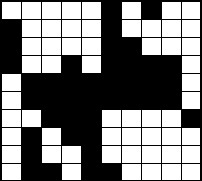
\includegraphics[width = \columnwidth]{./assets/y04s02-ai-homework-01-s02-report-p02.jpg}
            \caption{Пошкоджене зображення, подане на вхід мережі}
            \label{subfig:image-recovery-01}
          \end{subfigure}%
          \hspace{1\gridunitwidth}%
          \begin{subfigure}[t]{6\gridunitwidth - 0.5\gridunitwidth}
            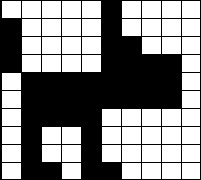
\includegraphics[width = \columnwidth]{./assets/y04s02-ai-homework-01-s02-report-p03.jpg}
            \caption{Вихідне зображення, відновлене до еталонного}
            \label{subfig:image-recovery-03}
          \end{subfigure}
          \caption{Приклад відновлення пошкодженого зображення}
          \label{fig:image-recovery}
        \end{figure}

      \subsubsection{Розпізнавання образів}
        В такому випадку виходить, що мережа Хопфілда відновлює початкове зображення~— еталон, тому іноді стверджують, що мережу використовують для розпізнавання образів. Однак, це не так. Щоб розв'язати задачу розпізнавання образів, інструмент повинен віднести вхідні данні до певної наперед заданої категорії, тобто класифікувати їх. Натомість, мережа Хопфілда не виконує цю задачу, а виключно відновлює інформацію, збережену всередині своїх нейронів, тому не зовсім коректно стверджувати, що мережу Хопфілда використовують для розв'язку задач розпізнавання образів.

      \subsubsection{Задачі оптимізації}
        Тим не менш, область використання мережі Хопфілда не обмежується збереженням і відновлення даних. Ці властивості дозволяють використати мережу для задач оптимізації на кшталт задачі комівояжера. Хопфілд і Тенк запропонували метод, суть якого полягає в тому, щоб представити тимчасовий розв'язок задачі як стан мережі з~$I = K^2$~нейронів, де~$K$~— кількість міст у поставленій задачі комівояжера. Тоді кожен нейрон представляє припущення, що в оптимальному маршруті саме це місто знаходиться на саме цьому кроці, і ця комбінація відповідає даному нейрону~(рис.~\ref{fig:hopfield-tsp}).

        \begin{figure}[!htbp]
          \centering
          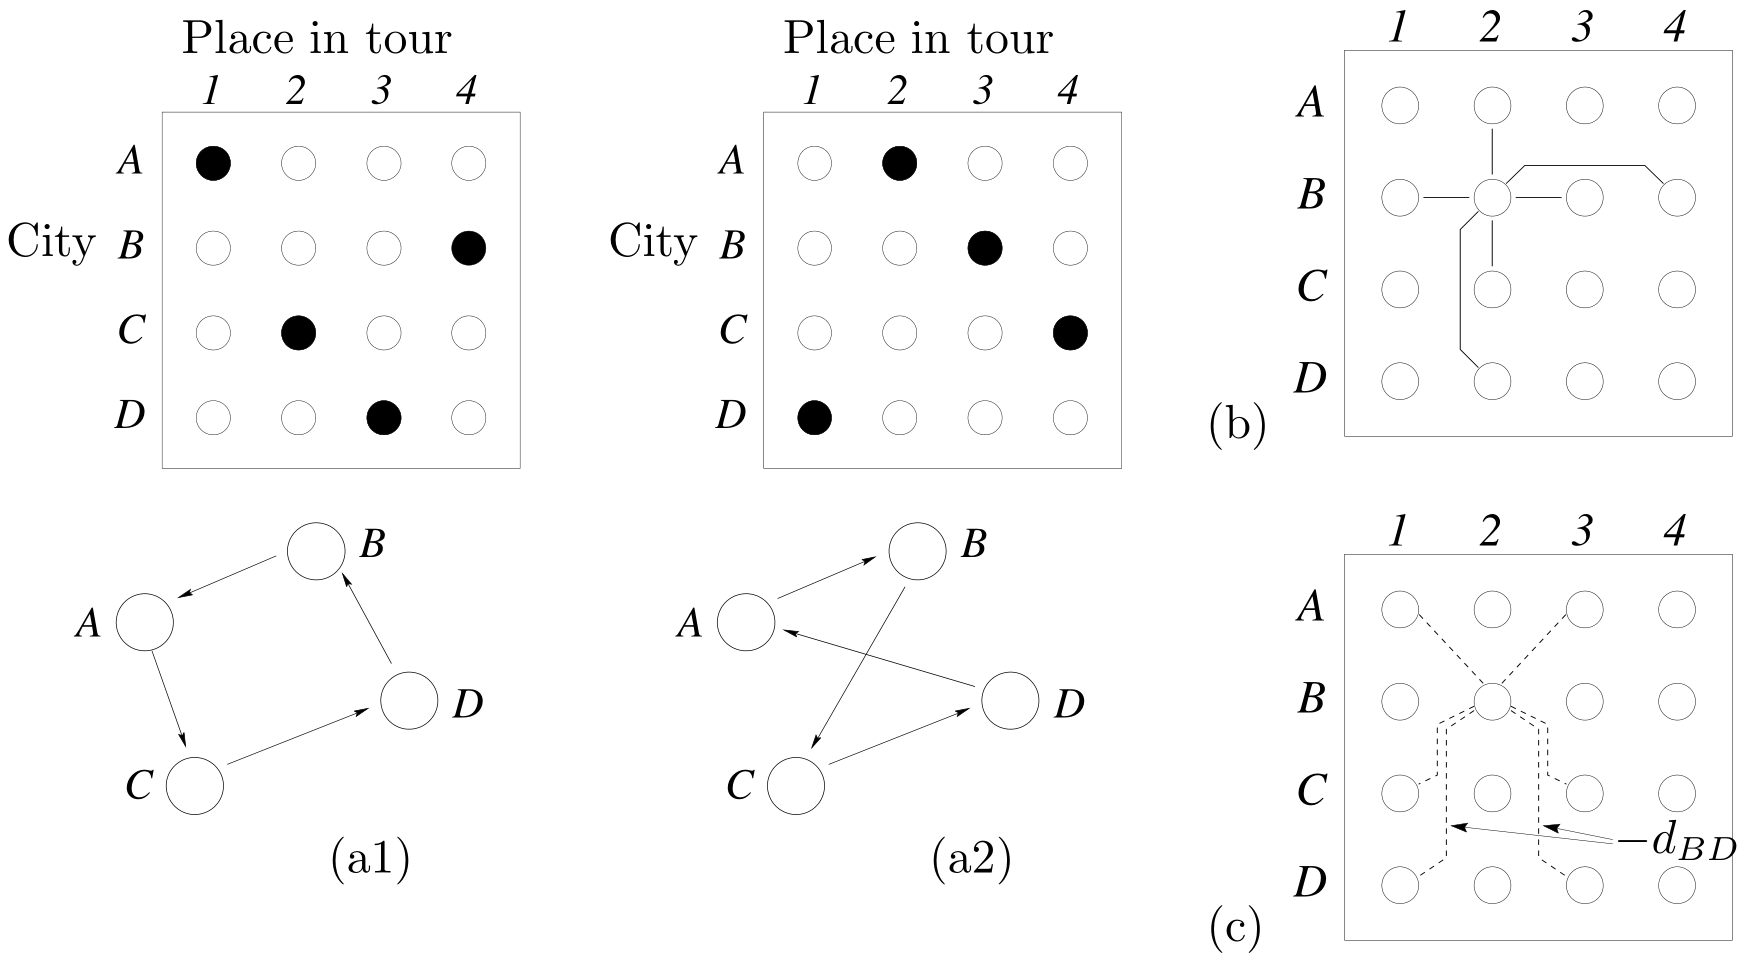
\includegraphics[width = 12\gridunitwidth]{./assets/y04s02-ai-homework-01-s02-report-p04.png}
          \caption{Представлення можливих розв'язків задачі комівояжера у вигляді станів мережі Хопфілда}
          \label{fig:hopfield-tsp}
        \end{figure}

        В такому випадку зручно представити стани нейронів як $0$ і $1$, а не $-1$ і $1$. Тоді ваги покажуть функцію енергії, яка буде мінімізована лише тоді, коли стан мережі є правильним маршрутом. Правильний стан мережі, який відповідає правильному маршруту,~— це такий стан, який виглядає як матриця перестановок, тобто в якій в кожному рядку і в кожній колонці є лише одне значення~«1». Щоб мережа слідувала цьому правилу, можна встановити великі від'ємні значення між усіма парами нейронів, які знаходяться в одному рядку або одній колонці. Також можна встановити додатне значення зсуву, щоб переконатись, що~$K$~нейронів увімкнуться. Таким чином, оскільки мережа Хопфілда прагне мінімізувати свою енергію, вона також повинна мінімізувати довжину маршруту між містами, які необхідно обійти.

    \subsection{Актуальність}
      Властивості мережі Хопфілда дозволяють застосовувати її у декількох сферах, однак широкий спектр застосувань не завжди означає актуальність. Перш за все, станом на 2020~рік, мережу Хопфілда майже не використовують для реалізації асоціативної пам'яті у широких застосуваннях. Найбільша потреба в асоціативній пам'яті є у процесорах та мережевих пристроях. В обох цих випадках найважливішими параметрами є швидкість роботи, кількість пам'яті, простота та вартість реалізації. На превеликий жаль, характеристикою нейронних мереж є висока складність, особливо порівняно з іншими методами на кшталт буферів асоціативної трансляції~(\transeng{translation lookaside buffers, \allcaps{TSB}}). Це призводить до низької надійності та високої вартості, тому мережа Хопфілда не отримала широкого розповсюдження у промислових застосуваннях.

      Друга область використання знаходиться на межі між корекцією помилок і розпізнаванням образів, наприклад, виправлення рукописного вводу. Використовуючи здатність мережі Хопфілда запам'ятовувати бажані стани, можна натренувати її на еталонні форми символів і використовувати для «розпізнавання» рукописного вводу. Однак, усі ці функції точніше, швидше і краще виконує інший тип нейронних мереж~— згорткові~(\transeng{convolutional neural networks, \allcaps{CNN}}), тому і тут мережа Хопфілда не отримала широкого застосування.

      Загалом, мережа Хопфілда є важливою академічною моделлю, яка підходить для того, щоб навчати студентів теорії штучних нейронних мереж.

  \section{Теоретичні відомості}
    Нейронна мережа Хопфілда визначається тим, що має повнозв'язну симетричну матрицю зв'язків. У процесі роботи динаміка таких мереж сходиться до одного з положень рівноваги. Ці положення рівноваги є локальними мінімумами функціоналу, який називається енергією мережі. На відміну від багатьох нейронних мереж, що працюють до отримання відповіді через певну кількість тактів, мережі Хопфілда працюють до досягнення рівноваги, коли наступний стан мережі дорівнює попередньому.

    \begin{figure}[!htbp]
      \centering
      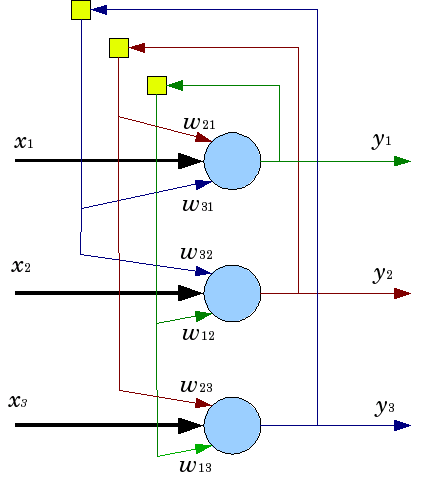
\includegraphics[width = 7\gridunitwidth]{./assets/y04s02-ai-homework-01-s02-report-p01.png}
      \caption{Приклад мережі Хопфілда}
      \label{fig:hopfield-net}
    \end{figure}

    Залежно від функції активації нейронів, порядку оновлення та деяких інших параметрів роботи мережі, розрізняють декілька варіацій, зокрема двійкову та неперервну мережі Хопфілда.

    \subsection{Двійкова мережа Хопфілда}
      Двійкова мережа Хопфілда — це частковий випадок неперервного режиму роботи мережі, однак саме його найчастіше використовують для вирішення задач розпізнавання образів, тому почнемо розгляд мережі на саме з цього режиму.

      \subsubsection{Архітектура}
      Позначимо зв'язок від нейрона~$j$ до нейрона~$i$ як~$w_{ij}$. Мережа Хопфілда складається з~$I$~нейронів. Зазвичай зв'язки між нейронами даної мережі підкорюються таким правилам:
      \begin{enumerate}
        \item Вони повністю зв'язані між собою за допомогою симетричних, двонаправлених зв'язків, тобто~$w_{ij} = w_{ji}$. Це правило гарантує, що під час застосування правила активації, енергія функції монотонно спадає~\cite{mackay-info-theory}. Інакше мережа може зациклюватись або вести себе хаотично.
        \item Всередині мережі відсутні зв'язки нейрона самого з собою, тобто для будь-якого~$i$ вага~$w_{ij} = 0$.
      \end{enumerate}

      Також у мережі можуть бути зсуви~(\transeng{bias}), які можна розглядати як зв'язки від нейрона~$0$, вихід якого завжди дорівнює~$x_0 = 1$. Вихід нейрона позначимо як~$x_i$, а сукупність усіх поточних значень виходів нейронів будемо називати станом мережі.

      \subsubsection{Оновлення і робота мережі}
        Грубо кажучи, правило роботи в двійковій мережі Хопфілда полягає в тому, щоб кожний нейрон оновлював свій стан, ніби він — єдиний нейрон, який має порогову функцію активації:
        \begin{IEEEeqnarray*}{rCl}
          x(a) \equiv \Theta(a) \equiv
          \left\{
          \begin{IEEEeqnarraybox}[
            \IEEEeqnarraystrutmode
            \IEEEeqnarraystrutsizeadd{2pt}{2pt}
          ][c]{r.s.l}
             1, & якщо $a \geqslant \theta_i$,\\
            -1, & у противному випадку.
          \end{IEEEeqnarraybox}
          \right.
        \end{IEEEeqnarray*}
        Тут~$\theta_i$~— це порогове значення. Коли зважена сума у нейроні набуває значення, яке більше за~$\theta_i$, нейрон активується.

        Всередині мережі Хопфілда є зворотній зв'язок, тобто вихід кожного нейрона є входом для усіх інших нейронів, тому необхідно зазначити порядок, у якому будуть виконуватись оновлення. Оновлення можуть бути:
        \begin{itemize}
          \item синхронними, коли спочатку усі нейрони оновлюють свої значення за формулою:
          \begin{IEEEeqnarray*}{rCl}
            a_i = \sum_j w_{ij} x_{j},
          \end{IEEEeqnarray*}
          а потім одночасно оновлюють свої стани до значення~$x_i$, яке розраховується так:
          \begin{IEEEeqnarray*}{rCl}
            x_i = \Theta(a_i)
          \end{IEEEeqnarray*}
        \item асинхронними, коли у певний момент часу лише один нейрон обчислює своє значення. Порядок обраних нейронів може бути зафіксованим або випадковим.
        \end{itemize}
        Залежно від типу оновлень, властивості мережі Хопфілда можуть змінюватись.

      \subsubsection{Енергія}
        Кожне оновлення мережі змінює її стан. Із кожним станом мережі Хопфілда пов'язана скалярна величина, яку називають енергією мережі~$E$. Вона обчислюється так:
        \begin{IEEEeqnarray*}{rCl}
          E = -\frac{1}{2} \sum_{i, j} w_{ij} x_i x_j
            + \sum_{i} \theta_i x_i
        \end{IEEEeqnarray*}
        Ця величина називається енергією, бо після того, як нейрони мережі оновлюються, енергія може зменшуватись або залишатись незмінною~(рис.~\ref{fig:energy}).

        \begin{figure}[!htbp]
          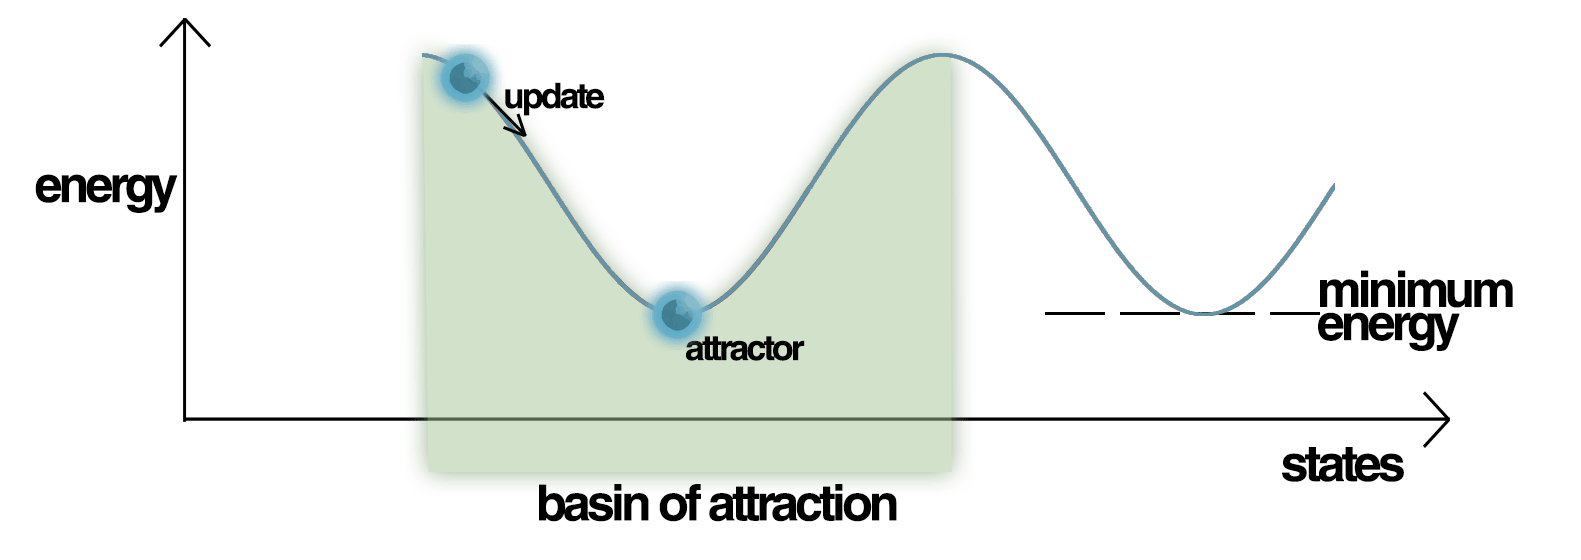
\includegraphics[width = 12\gridunitwidth]{./assets/y04s02-ai-homework-01-s02-report-p05.png}
          \caption{Ландшафт енергії мережі Хопфілда, який показує поточний стан мережі (на горі), притягаючий стан, до якого так чи інакше зійдеться мережа, та впадину притяжіння, відтінену зеленим кольором}
          \label{fig:energy}
        \end{figure}

        Крім того, після повторних оновлень мережа так чи інакше зійдеться до стану, який є локальним мінімумом функції енергії. Отже, якщо стан мережі відповідає локальному мінімуму функції енергії, він вважається стабільним станом мережі.

      \subsubsection{Тренування мережі}
        Штучні нейронні мережі тренують за допомогою правил навчання. Існують різні правила навчання нейронних мереж, але бажано, щоб правило навчання мало такі 2~властивості:
        \begin{enumerate}
          \item Локальність. Правило навчання вважається локальним, якщо для оновлення ваги кожного нейронного зв'язку достатньо лише тої інформації, яка міститься виключно у тих нейронах, що з'єднані цим зв'язком.
          \item Інкрементальність. Правило навчання вважається інкрементальним, коли з його допомогою мережа може вивчити нові поняття, не використовуючи інформацію про поняття, які вона вивчила раніше. Тобто для того, щоб оновити ваги зв'язків для вивчення нового поняття, мережі вистачить лише минулих значень ваг та власне нового поняття.
        \end{enumerate}

        Одним з правил навчання, які мають обидві вищезазначені властивості, є правило Хебба, яке часто застосовують для тренування мережі Хопфілда. Як відомо, правило навчання оновлює ваги зв'язків між нейронами мережі таким чином, щоб мережа вчилась певним поняттям.

        У нейронній мережі Хопфілда кожен факт представляється як двійковий набір даних~$\mathbf{x}$, де~$x_{i} \in \{-1, 1\}$, тому правило навчання має зробити множину~$\{\mathbf{x}^{(n)}\}$, яка містить факти, що треба закріпити, стабільними станами мережі. Щоб зробити будь-які стани стабільними, тобто «записати» факти у мережу, необхідно зменшувати енергію, яку набуватиме нейронна мережа при переході до бажаного стану.

        Щоб зменшувати енергію бажаних станів, необхідно оновлювати ваги зв'язків між нейронами відповідним способом, тому за правилом Хебба для мережі Хопфілда ваги зв'язків між нейронами встановлюються так:
        \begin{IEEEeqnarray*}{rCl}
          w_{ij} = \eta \sum_{n} x_{i}^{(n)} x_{j}^{(n)},
        \end{IEEEeqnarray*}
        де~$\eta$~— певна неважлива константа. Щоб попередити ситуацію, при якій найбільша вага буде рости разом зі значенням~$N$, можна обрати значення константи~$\eta = 1 / N$.

        Ваги зв'язків між нейронами істотно впливають на значення виходів нейронів та навчання мережі. У мережі Хопфілда вони симулюють тяжіння та відштовхування нейронів між собою. Наприклад, розглянемо вагу між нейронами~$i$ і~$j$, яка позначається~$w_{ij}$. Якщо вага~$w_{ij} > 0$, правило активації означає, що:
        \begin{itemize}
          \item коли значення нейрона~$x_{j} = 1$, нейрон~$j$ збільшує зважену суму, отже, нейрон~$j$ притягує значення нейрона $x_i$ до значення~$x_i = 1$.
          \item коли значення нейрона~$x_{j} = -1$, нейрон~$j$ зменшує зважену суму, отже, нейрон~$j$ відштовхує значення нейрона $x_i$ до значення~$x_i = -1$.
        \end{itemize}
        Таким чином, значення нейронів~$i$ і~$j$ будуть збігатись, якщо вага зв'язку між ними додатна, і, навпаки, розбігатись, якщо вага від'ємна.

  \section{Реалізація}
    Описавши теоретичні відомості про мережу Хопфілда, використаємо її реалізацію~\cite{tyamamoto-hopfield} для вирішення задач, які найбільше схожі на розпізнавання зображення. Першою такою задачею буде відновлення пошкодженого початкового зображення. Тоді порядок роботи програми виглядатиме так:
    \begin{enumerate}
      \item Запам'ятати вхідні зображення.
      \item Внести випадкові пошкодження в еталонне зображення.
      \item Подати пошкоджене зображення на вхід нейронної мережі.
      \item Запустити нейронну мережу.
      \item Коли мережа зійдеться до стабільного стану, вивести результат.
    \end{enumerate}

    Наступний режим роботи реалізації, який в контексті даного завдання можна розуміти як розпізнавання зображень~— це відновлення рукописних цифр. В якості тренувальних даних, тобто набору рукописних цифр, використаємо деякі цифри із набору даних~\textenglish{\allcaps{MNIST}}. При цьому програма не буде класифікувати цифри, адже нейронна мережа Хопфілда не призначена для категоризації вхідних даних. Тем не менш, вона зможе відновити більшість вхідних рукописних цифр до значень, схожих на еталонні. У цьому випадку порядок роботи програмної реалізації буде аналогічним.

    Отже, щоб використати реалізацію, встановлюємо її залежності, запускаємо і тренуємо. Під час роботи програми отримаємо результат у вигляді графічних звітів~(рис.~\ref{fig:image-recovery-py}).

    \begin{figure}[!htb]
      \begin{subfigure}[t]{6\gridunitwidth - 0.5\gridunitwidth}
        \centering
        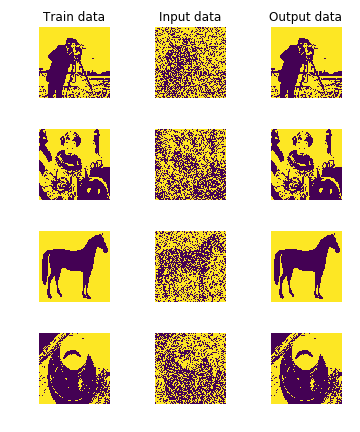
\includegraphics[width = 6\gridunitwidth]{./assets/y04s02-ai-homework-01-s02-report-p06.png}
        \caption{Відновлення пошкодженого зображення}
        \label{subfig:image-recovery-py-01}
      \end{subfigure}%
      \hspace{1\gridunitwidth}
      \begin{subfigure}[t]{6\gridunitwidth - 0.5\gridunitwidth}
        \centering
        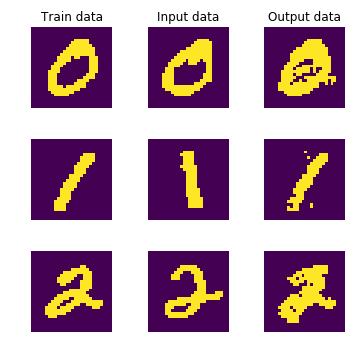
\includegraphics[width = 6\gridunitwidth]{./assets/y04s02-ai-homework-01-s02-report-p07.png}
        \caption{Відновлення рукописних цифр}
        \label{subfig:image-recovery-py-02}
      \end{subfigure}%
      \caption{Результати роботи реалізації мережі Хопфілда}
      \label{fig:image-recovery-py}
    \end{figure}

    Як видно з результатів відновлення зображень~(рис.~\ref{subfig:image-recovery-py-01}), реалізована нейронна мережа здатна досить точно відновити 4~пошкоджених еталонних зображень, причому варто зазначити, що вхідні дані були суттєво змінені випадковими даними.

    Що до відновлення рукописних цифр, результати менш вражаючі~(рис.~\ref{subfig:image-recovery-py-02}): видно, що мережа намагалась відновити еталонні зображення, однак в процесі відновлення створила навіть більше артефактів, ніж на вхідних даних. Оскільки результати роботи мережі не повернулись до точного еталонного стану, їх не можна точно порівняти з еталонними і визначити, що вхідні дані належать певному класу. Отже, мережі бракує точності, щоб використовувати її для задачі розпізнавання зображень.

  \clearpage
  \section*{Висновки}
  \addcontentsline{toc}{section}{Висновки}
    Виконуючи дане домашнє завдання, ми ознайомились із нейронною мережею Хопфілда, дослідили області її використання, актуальність, архітектуру та принцип роботи, а також використали реалізацію, щоб розв'язати завдання, суміжні з розпізнаванням зображень.

    Визначено, що нейронна мережа Хопфілда може бути використана як асоціативна пам'ять, тобто пам'ять, яка дозволяє відновити повний зміст певної інформації лише за її частиною. Також мережу Хопфілда можна використати як фільтр, який коригуватиме помилки у вхідній інформації так, щоб вона співпадала з еталонною. Крім цього, мережа Хопфілда може евристично розв'язувати задачі оптимізації на кшталт задачі комівояжера. Для цього достатньо представити задачу у форматі, зручному для роботи мережі.

    Незважаючи на те, що мета домашнього завдання полягала у дослідженні роботи мережі Хопфілда для розпізнавання зображень, виявилось, що вона взагалі не може розв'язувати ці задачі у їх строгому формулюванні. Річ у тім, що мережа Хопфілда не здатна відносити вхідні дані до певного класу~— вона може виключно відновлювати їх до певного стабільного стану. Так, цей стан можна задати параметрично, як це потрібно для розв'язання задачі комівояжера, але цю властивість неможливо застосувати для класифікації даних, і тому після відновлення еталонного зображення класифікація буде окремою і часто дуже складною задачею.

    Також було виявлено, що мережа Хопфілда не отримала широкого розповсюдження у повсякденних застосуваннях. Для реалізації асоціативної пам'яті у сучасних пристроях, які її потребують, мережу витіснили асоціативні буфери трансляції; як для реалізації асоціативної структури даних у програмі, то нейронна мережа буде занадто складною. Із задачами розпізнавання образів значно краще справляються згорткові нейронні мережі, тому станом на 2020~рік вони отримали найбільше розповсюдження для їх розв'язання. В задачах оптимізації зазвичай використовуються інші алгоритми, не пов'язані з машинним навчанням, на кшталт симплекс-метода, метода Нелдера—Меда та еліпсоїдного метода. Тому можна зробити висновок, що мережа Хопфілда актуальна лише для навчання людей основам нейронних мереж.

    Ще у домашньому завданні були викладені теоретичні відомості про мережу Хопфілда, а згодом на їх основі був показаний приклад роботи мережі для розв'язання задач, що найближче схожі на задачі розпізнавання образів. Результати роботи вкотре підкреслили, що нейронна мережа Хопфілда підходить виключно для відновлення початкових даних, але не є повноцінним рішенням для розпізнавання зображень.

  % Bibliography
  \addcontentsline{toc}{section}{Література}
  \printbibliography

  \appendix
  \section{Лістинг реалізації}
    \inputpython{../s01-solution/Hopfield-Network-master/network.py}{Файл~\textenglish{\filename{network.py}}}{lst:network.py}
    \inputpython{../s01-solution/Hopfield-Network-master/train.py}{Файл~\textenglish{\filename{train.py}}}{lst:network.py}
    \inputpython{../s01-solution/Hopfield-Network-master/train_mnist.py}{Файл~\textenglish{\filename{train\_mnist.py}}}{lst:network.py}

\end{document}
